% This is "aamas2011.tex" August 2011
% This file should be compiled with "aamas2011.cls" 
% This example file demonstrates the use of the 'aamas2011.cls'
% LaTeX2e document class file. It is for those submitting
% articles to AAMAS 2011 conference. This file is based on
% the sig-alternate.tex example file.
% The 'sig-alternate.cls' file of ACM will produce a similar-looking,
% albeit, 'tighter' paper resulting in, invariably, fewer pages.
% than the original style ACM style.
%
% ----------------------------------------------------------------------------------------------------------------
% This .tex file (and associated .cls ) produces:
%       1) The Permission Statement
%       2) The Conference (location) Info information
%       3) The Copyright Line with AAMAS data
%       4) NO page numbers
%
% as against the acm_proc_article-sp.cls file which
% DOES NOT produce 1) thru' 3) above.
%
% Using 'aamas2011.cls' you don't have control
% from within the source .tex file, over both the CopyrightYear
% (defaulted to 200X) and the IFAAMAS Copyright Data
% (defaulted to X-XXXXX-XX-X/XX/XX).
% These information will be overwritten by fixed AAMAS 2011 information
% in the style files - it is NOT as you are used with ACM style files.
%
% ---------------------------------------------------------------------------------------------------------------
% This .tex source is an example which *does* use
% the .bib file (from which the .bbl file % is produced).
% REMEMBER HOWEVER: After having produced the .bbl file,
% and prior to final submission, you *NEED* to 'insert'
% your .bbl file into your source .tex file so as to provide
% ONE 'self-contained' source file.
%

% This is the document class for full camera ready papers and extended abstracts repsectively 

\documentclass{aamas2011}

% if you are using PDF LaTex and you cannot find a way for producing
% letter, the following explicit settings may help

\pdfpagewidth=8.5truein
\pdfpageheight=11truein



% Use the postscript times font!
\usepackage{times}

% the following package is optional:
\usepackage{latexsym} 
\usepackage{amsmath}
\usepackage{amssymb}
\usepackage{subfigure}

% Load pfg package for drawing transition systems
\usepackage{xspace}
\usepackage{url}

\usepackage{tikz,pgf,pgfplots}
\usetikzlibrary{calc,arrows,automata,trees,shapes,plotmarks}


\usepackage{algorithm}
\usepackage{algorithmic}
%\usepackage[ruled,vlined]{algorithm2e}

\usepackage{textcomp}

% \usepackage[sort&compress,numbers]{natbib}

%% How deep we want to number sections/subsections
\setcounter{secnumdepth}{1}  


% \renewcommand{\baselinestretch}{0.965}

\usepackage{comment}



%%%%%%%%%%%%%%%%%%%%%%%%%%%%%%%%%%%%%%%%%%%%%%%%%%%%%%%%%%%%%%%%%%%%%%%%
%%%%% START OF MACROS
%%%%%%%%%%%%%%%%%%%%%%%%%%%%%%%%%%%%%%%%%%%%%%%%%%%%%%%%%%%%%%%%%%%%%%%%
%%%%%%%%%%%%%%%%%%%%%%%%%%%%%%%%%%%%%%%%%%%%%%%%%%%%
% PERSONAL LaTex MACROS 
%	SEBASTAN SARDINA -- ssardina@cs.rmit.edu.au
%%%%%%%%%%%%%%%%%%%%%%%%%%%%%%%%%%%%%%%%%%%%%%%%%%%%



%%%%%%%%%%%%%%%%%%%%%%%%%%%%%%%%%%%%%%%%%%%%%%%%%%%%
% Font modes & definitions
%%%%%%%%%%%%%%%%%%%%%%%%%%%%%%%%%%%%%%%%%%%%%%%%%%%%

% conditional math environment
% \gdef\Math#1{\ifmmode #1 \else \mbox{$#1$}\fi}
\newcommand{\Math}[1]{\ensuremath{#1}}



\newcommand{\modesf}[1]{{\Math{\mathsf{#1}}}}
\newcommand{\modecal}[1]{{\Math{\mathcal{#1}}}}
\newcommand{\modeit}[1]{{\Math{\mathit{#1}}}}


\newcommand{\textmath}[1]{{\mbox{\textit{#1}}}}


%%%%%%%%%%%%%%%%%%%%%%%%%%%%%%%%%%%%%%%%%%%%%%%%%%%%
% Proper names
%%%%%%%%%%%%%%%%%%%%%%%%%%%%%%%%%%%%%%%%%%%%%%%%%%%%
\newcommand{\propername}[1]{\mbox{\small \textsf{#1}}}

\newcommand{\Golog}{\propername{Golog}}
\newcommand{\GologSpeak}{\propername{GologSpeak}}
\newcommand{\DGolog}{\propername{DGolog}}
\newcommand{\sGolog}{\propername{sGolog}}
\newcommand{\ConGolog}{\propername{ConGolog}}
\newcommand{\IndiGolog}{\propername{IndiGolog}}
\newcommand{\LeGolog}{\propername{LeGolog}}
\newcommand{\DTGolog}{\propername{DTGolog}}
\newcommand{\Prolog}{\propername{Prolog}}
\newcommand{\AgentSpeak}{\propername{AgentSpeak}}
\newcommand{\JASON}{\propername{Jason}}
\newcommand{\CANMINUS}{\propername{\CAN$^{\A}$}}
\newcommand{\CANMINUST}{\propernametiny{Can$^{\cal C}$}}
\newcommand{\CAN}{\propername{CAN}}
\newcommand{\CANT}{\propernametiny{Can}}
\newcommand{\CANPLAN}{\propername{CANPlan}}
\newcommand{\CANPLANT}{\propernametiny{CanPlan}}
\newcommand{\CANPLANII}{\propername{CanPlan2}}
\newcommand{\CANPLANOR}{\propername{Can(Plan)}}
\newcommand{\CANGOAL}{\propername{CanGoal}}
\newcommand{\JACK}{\propername{JACK}}
\newcommand{\weka}{\propername{weka}}
\newcommand{\JACKTM}{\propername{Jack\texttrademark}}
\newcommand{\JAM}{\propername{JAM}}
\newcommand{\DAPL}{\propername{2APL}}
\newcommand{\GOAL}{\propername{GOAL}}
\newcommand{\PRS}{\propername{PRS}}
\newcommand{\SPARK}{\propername{SPARK}}
\newcommand{\RAP}{\propername{Rap}}
\newcommand{\dMARS}{\propername{dMARS}}
\newcommand{\TAPL}{\propername{3APL}}
\newcommand{\GOALBDI}{\propername{GOAL}}
\newcommand{\JSHOP}{\propername{JSHOP}}
\newcommand{\JSHOPII}{\propername{JSHOP2}}
\newcommand{\ASHOP}{\propername{A-SHOP}}
\newcommand{\SHOP}{\propername{SHOP}}
\newcommand{\SHOPII}{\propername{SHOP2}}
\newcommand{\ACT}{\propername{ACT}}
\newcommand{\SIPEII}{\propername{SIPE-2}}
\newcommand{\OPLANII}{\propername{O-PLAN2}}
\newcommand{\Retsina}{\propername{Retsina}}
\newcommand{\IPEM}{\propername{IPEM}}
\newcommand{\SAGE}{\propername{Sage}}
\newcommand{\DECAF}{\propername{Decaf}}
\newcommand{\PROPICE}{\propername{Propice-Plan}}
\newcommand{\CYPRESS}{\propername{Cypress}}
\newcommand{\CPEF}{\propername{CPEF}}
\newcommand{\JADEX}{\propername{JADEX}}
\newcommand{\IMPACT}{\propername{IMPACT}}
\newcommand{\PDT}{\propername{PDT}}


%%%%%%%%%%%%%%%%%%%%%%%%%%%%%%%%%%%%%%%%%%%%%%%%%%%%
% Calligraphic letters - Taken from Giuseppe De Giacomo 2006
%%%%%%%%%%%%%%%%%%%%%%%%%%%%%%%%%%%%%%%%%%%%%%%%%%%%
\newcommand{\A}{\modecal{A}} \newcommand{\B}{\modecal{B}}
\newcommand{\C}{\modecal{C}} \newcommand{\D}{\modecal{D}}
\newcommand{\E}{\modecal{E}} \newcommand{\F}{\modecal{F}}
\newcommand{\G}{\modecal{G}} \renewcommand{\H}{\modecal{H}}
\newcommand{\I}{\modecal{I}} \newcommand{\J}{\modecal{J}}
\newcommand{\K}{\modecal{K}} \renewcommand{\L}{\modecal{L}}
\newcommand{\M}{\modecal{M}} \newcommand{\N}{\modecal{N}}
\renewcommand{\O}{\modecal{O}} \renewcommand{\P}{\modecal{P}}
\renewcommand{\S}{\modecal{S}} \newcommand{\T}{\modecal{T}}
\newcommand{\U}{\modecal{U}} \newcommand{\V}{\modecal{V}}
\newcommand{\W}{\modecal{W}} \newcommand{\X}{\modecal{X}}
\newcommand{\Y}{\modecal{Y}} \newcommand{\Z}{\modecal{Z}}
\newcommand{\R}{\modecal{R}} 



%%%%%%%%%%%%%%%%%%%%%%%%%%%%%%%%%%%%%%%%%%%%%%%%%%%%
% Situation Calculus macros
%%%%%%%%%%%%%%%%%%%%%%%%%%%%%%%%%%%%%%%%%%%%%%%%%%%%

% Sitcalc Golog/ConGolog/IndiGolog programs
\newcommand{\mif}{\mbox{\bf if}}
\newcommand{\mwhile}{\mbox{\bf while}}
\newcommand{\mreturn}{\mbox{\bf return}}
\newcommand{\mthen}{\mbox{\bf then}}
\newcommand{\melse}{\mbox{\bf else}}
\newcommand{\mdo}{\mbox{\bf do}}
\newcommand{\mnoOp}{\mbox{\bf $noOp$}}
\newcommand{\mproc}{\mbox{\bf proc}}
\newcommand{\mend}{\mbox{\bf end}}
\newcommand{\mendproc}{\mbox{\bf endProc}}
\newcommand{\mendif}{\mbox{\bf endIf}}
\newcommand{\mendwhile}{\mbox{\bf endWhile}}
\newcommand{\mendfor}{\mbox{\bf endFor}}
\newcommand{\mfor}{\mbox{\bf for}}
\def\prparallel{\mathrel{\rangle\!\rangle}}
\def\supparallel{\mathord{|\!|}}
\newcommand{\conc}{\mbox{$\parallel$}}
\newcommand{\pconc}{\mbox{$\prparallel$}}
\newcommand{\search}{\mbox{$\Sigma$}}
\newcommand{\searchO}{\mbox{$\Sigma_o$}}
\newcommand{\searchOM}{\mbox{$\Sigma_o^M$}}
\newcommand{\searchCR}{\mbox{$\Sigma_{cr}$}}
\newcommand{\searchR}{\mbox{$\Sigma_{r}$}}
\newcommand{\searchM}{\mbox{$\Sigma^M$}}
\newcommand{\searchC}{\mbox{$\Sigma_c$}}
\newcommand{\searchCM}{\mbox{$\searchC^M$}}
\newcommand{\searchCB}{\mbox{$\Sigma_{cb}$}}
\newcommand{\searchD}{\mbox{$\Delta$}}
\newcommand{\searchE}{\mbox{$\Delta_e$}}
\newcommand{\searchEM}{\mbox{$\Delta_e^M$}}
\newcommand{\searchL}{\mbox{$\Delta_l$}}
\newcommand{\searchER}{\mbox{$\Delta_r$}}
\newcommand{\searchERM}{\mbox{$\Delta_r^M$}}
\newcommand{\mnt}{\mbox{$mnt$}}


%%% Knowledge in sitcalc
\newcommand{\Know}{\mbox{\bf Know}}
\newcommand{\KWhether}{\mbox{\bf KWhether}}
\newcommand{\Kref}{\mbox{\bf KRef}}
\newcommand{\nows}{{\hbox{\small\sf now}}}
\newcommand{\now}{{\mbox{\sf now}}}


% IndiGolog macros
\newcommand{\Sensed}{\textmath{Sensed}}
\newcommand{\hend}{\textmath{end}}
\newcommand{\Trans}{\textmath{Trans}}
\newcommand{\Final}{\textmath{Final}}
\newcommand{\Poss}{\textmath{Poss}}
\newcommand{\Transobs}{\textmath{TransObs}}


%%%%%%%%%%%%%%%%%%%%%%%%%%%%%%%%%%%%%%%%%%%%%%%%%%%%
% CAN notation for BDI Agents
%%%%%%%%%%%%%%%%%%%%%%%%%%%%%%%%%%%%%%%%%%%%%%%%%%%%
\newcommand{\Goal}{\modesf{Goal}}
\newcommand{\GoalS}{\modesf{G}}
\newcommand{\SGoal}{\modesf{SGoal}}
\newcommand{\SGoalS}{\modesf{SG}}
\newcommand{\goal}[3]{{\sf Goal}(#1,#3,#2)}
\newcommand{\goalp}[3]{{\sf Goal}_{P}(#1,#3,#2)}
\newcommand{\goalsfp}{\goal{s}{f}{P}}
\newcommand{\goalsfpp}{\goalp{s}{f}{P}}
\newcommand{\goalt}[2]{{\sf Goal}(#1,#2)}
\newcommand{\goalsf}{\goal{s}{f}}

\newcommand{\Plan}{\modesf{Plan}}
\newcommand{\PlanP}{\modesf{P}}
\newcommand{\PlanArg}[1]{\Plan(#1)}

\newcommand{\pnil}{\mbox{\textit{nil}}}
\newcommand{\ptrue}{\mbox{\textit{true}}}
\newcommand{\pfalse}{\mbox{\textit{false}}}
\newcommand{\pfail}{\mbox{\textit{fail}}}

\newcommand{\pguardaltl}[1]{\mbox{$\altl #1 \altr$}} % guarded alternatives
\newcommand{\altl}{\llparenthesis}
\newcommand{\altr}{\rrparenthesis}

%% Macro for BDI plan rules:  \plane{a:b<-c} \plans{a<-c}
\newcommand\plane[1]{\planeaux!#1!}
\def\planeaux!#1:#2<-#3!{\Math{#1 \mbox{\rm:} #2\; \leftarrow #3}}
\newcommand\plans[1]{\planeaux!#1!}
\def\planeaux!#1<-#2!{\Math{#1 \leftarrow #2}}




%%%%%%%%%%%%%%%%%%%%%%%%%%%%%%%%%%%%%%%%%%%%%%%%%%%%
% START - Operational semantics
%%%%%%%%%%%%%%%%%%%%%%%%%%%%%%%%%%%%%%%%%%%%%%%%%%%%
% Labels
\newcommand{\bdi}{bdi}
\newcommand{\htn}{plan}
\newcommand{\transitionlabel}[1]{\modesf{{#1}}}

% Meta-transition
\newcommand{\mtransition}{\Longrightarrow} % meta transition
\newcommand{\mtransitionstar}{\overset{*}{\mtransition}} % trans meta closure
\newcommand{\mtransitiontype}[1]{\overset{\transitionlabel{#1}}{\mtransition}}
\newcommand{\mtransitionstartype}[1]{\overset{*}{\mtransitiontype{#1}}}

% Transition
\newcommand{\transition}{\longrightarrow} 	% regular transition

\newcommand{\transitionstar}{\overset{*}{\transition}} % trans closure
\newcommand{\transitionst}{\overset{*}{\transition}} %trans closure
\newcommand{\transitionanot}[1]{\transition_{#1}} 	% regular transition
\newcommand{\transitionbdistarint}
	{\overset{\transitionlabel{\bdi}_{*}}{\transition_i}}

\newcommand{\transitiontype}[1]{\overset{\transitionlabel{#1}}{\transition}}
\newcommand{\transitionbdi}{\overset{\transitionlabel{\bdi}}{\transition}}
\newcommand{\transitionhtn}{\overset{\transitionlabel{\htn}}{\transition}}
\newcommand{\transitionhtnstar}
	{\overset{\transitionlabel{\htn}_{*}}{\transition}}
\newcommand{\transitionbdistar}
{\overset{\transitionlabel{\bdi}_{*}}{\transition}}

\newcommand{\transitionhtnk}[1]
{\overset{\transitionlabel{\htn}_{#1}}{\transition}}
\newcommand{\transitionbdik}[1]
{\overset{\transitionlabel{\bdi}_{#1}}{\transition}}



%%%%%%%%%%%%%%%%%%%%%%%%%%%%%%%%%%%%%%%%%%%%%%%%%%%%
% Several notations
%%%%%%%%%%%%%%%%%%%%%%%%%%%%%%%%%%%%%%%%%%%%%%%%%%%%

%%%%%%%%%%%%%%%%%%%%%%%%%% Delimiters
\newcommand{\quotes}[1]{{\lq\lq #1\rq\rq}}
\newcommand{\set}[1]{\{#1\}}                      % set
\newcommand{\Set}[1]{\left\{#1\right\}}
\newcommand{\bigmid}{\Big|}
\newcommand{\card}[1]{|{#1}|}                     % cardinality of a set
\newcommand{\Card}[1]{\left| #1\right|}
\newcommand{\cards}[1]{\sharp #1}
\newcommand{\sub}[1]{[#1]}
\newcommand{\tuple}[1]{\Math{\langle #1 \rangle}}		% tuple
\newcommand{\Tuple}[1]{\Math{\left\langle #1 \right\rangle}}		% tuple
\newcommand{\tup}[1]{\tuple{#1}}            			% tuple
\newcommand{\Tup}[1]{\Tuple{#1}}
\newcommand{\config}[1]{\tuple{#1}}	% configuration

% A symbol with something on top and under: \underoverset{under}{above}{text}
\newcommand{\underoverset}[3]{\underset{#1}{\overset{#2}{#3}}}


\newcommand{\myi}{\emph{(i)}\xspace}
\newcommand{\myii}{\emph{(ii)}\xspace}
\newcommand{\myiii}{\emph{(iii)}\xspace}
\newcommand{\myiv}{\emph{(iv)}\xspace}
\newcommand{\myv}{\emph{(v)}\xspace}
\newcommand{\myvi}{\emph{(vi)}\xspace}


%%%%%%%%%%%%%%%%%%%%%%%%%%%%%%%%%%%%%%%%%%%%%%%%%%%%
% Several useful symbols
%%%%%%%%%%%%%%%%%%%%%%%%%%%%%%%%%%%%%%%%%%%%%%%%%%%%

% Symbols
\newcommand{\powerset}{\mathbb{P}}
\newcommand{\NatN}{\Math{\mathbb{N}_0}} % naturals+0
\newcommand{\Nat}{\Math{\mathbb{N}}}
\newcommand{\mgu}{\modesf{mgu}}
\newcommand{\complexsub}{\modesf{cplex}}

% True and False
\newcommand{\true}{\mathtt{true}}
\newcommand{\false}{\mathtt{false}}
\newcommand{\True}{\mathtt{True}}
\newcommand{\False}{\mathtt{False}}
% \newcommand{\TRUE}{\uppercase{\true}}
% \newcommand{\FALSE}{\uppercase{\false}}

% LTL modalities
\newcommand{\mnext}{\bigcirc}		% next
\newcommand{\malways}{\square}		% always
\newcommand{\meventually}{\lozenge}	% eventually
\newcommand{\muntil}{\mathop{\U}}	% until

% Relations
\newcommand{\goto}[1]{\stackrel{#1}{\longrightarrow}}
\newcommand{\gotoii}[2]{\underoverset{#2}{#1}{\longrightarrow}}
\newcommand{\isdef}{\hbox{$\stackrel{\mbox{\tiny def}}{=}$}}

%%%%%%%%%%%%%%%%%%%%%%%%%%%%%%%%%%%%%%%%%%%%%%%%%%%%
% Macros for Proofs
%%%%%%%%%%%%%%%%%%%%%%%%%%%%%%%%%%%%%%%%%%%%%%%%%%%%

% Proofs symbols: provided by amsmath package now as \qed
\newcommand{\qedblack}{\phantom{a} \hfill \ensuremath{\blacksquare}}



\long\def\eatpar#1{%
\ifx#1\par                      % se il token e' \par
\let\nextmove=\eatpar           % rimetti \eatpar in coda
\else
\let\nextmove=#1%               altrimenti, rimetti il token in coda
\fi
\nextmove%                      il token o \eatpar viene rimesso in coda
}

\def\qed{\hfill{\qedboxempty}      % qed with empty box
  \ifdim\lastskip<\medskipamount \removelastskip\penalty55\medskip\fi}

\def\qedboxempty{\vbox{\hrule\hbox{\vrule\kern3pt
                 \vbox{\kern3pt\kern3pt}\kern3pt\vrule}\hrule}}

\def\qedfull{\hfill{\qedboxfull}   % qed with full box
  \ifdim\lastskip<\medskipamount \removelastskip\penalty55\medskip\fi}

\def\qedboxfull{\vrule height 4pt width 4pt depth 0pt}

\newcommand{\markfull}{\qedfull}
\newcommand{\markempty}{\qed}


%%%%%%%%%%%%%%%%%%%%%%%%%%%%%%%%%%%%%%%%%%%%%%%%%%%%
% Several special text abbreviations
%%%%%%%%%%%%%%%%%%%%%%%%%%%%%%%%%%%%%%%%%%%%%%%%%%%%

% Italic-text abbreviations (sets, etc.)
\newcommand{\CNF}{\modeit{CNF}}
\newcommand{\Actions}{\modeit{Act}}
\newcommand{\Events}{\modeit{Event}}
\newcommand{\freeVar}{\modeit{dom}}
\newcommand{\variant}{\modesf{ren}}
\newcommand{\Init}{\modeit{Init}}

\newcommand{\dummytask}{\mbox{\textit{dummyTask}}}


\newcommand{\BDI}{\mbox{BDI}}

\newcommand{\Active}{\modeit{Act}}






%%%%%%%%%%%%%%%%%%%%%%%%%%%%%%%%%%%%%%%%%%%%%%%%%%%%
% Margin notes for comments  
%%%%%%%%%%%%%%%%%%%%%%%%%%%%%%%%%%%%%%%%%%%%%%%%%%%%
\setlength{\marginparwidth}{0.1in}
\let\oldmarginpar\marginpar
\renewcommand\marginpar[1]{\-\oldmarginpar[\raggedleft\footnotesize #1]%
{\raggedright\footnotesize #1}}

\setlength{\marginparwidth}{0.5in}
\newcommand{\notem}[1]{\marginpar{\scriptsize  \textbf{#1}}}
\newcommand{\notems}[1]{\notem{S: #1}}
\newcommand{\noteml}[1]{\notem{L: #1}}
\newcommand{\notemd}[1]{\notem{D: #1}}

\newcommand{\ncheck}{\notem{CHECK!}}
\newcommand{\GGG}{\notem{GGG}}
\newcommand{\SSS}{\notem{SSS}}
\newcommand{\LIN}{\notem{LP}}
\newcommand{\YVES}{\notem{YL}}




%%%%%%%%%%%%%%%%%%%%%%%%%%%%%%%%%%%%%%%%%%%%%%%%%%%%
% PhD boxed notes for the committee in Toronto -- Taken from Ron Petrick 2004
%%%%%%%%%%%%%%%%%%%%%%%%%%%%%%%%%%%%%%%%%%%%%%%%%%%%
% \usepackage{color}
\newcounter{countphdnote}
% \newcommand{\phdnote}[1]{\textbf{#1}}
% \newcommand{\phdnote}[1]{
% \begin{center}
% \begin{tabular}{c}
% 	\begin{minipage}{4in}
% 		\fcolorbox{black}{black}{\textcolor
%     		{white}{\textbf{\ Note \thecountphdnote\ }}}
% 	\end{minipage} \\
%     	\fcolorbox{black}{white}{
% 	\begin{minipage}{6in}
% 		#1\addtocounter{countphdnote}{1}%
%     	\end{minipage}}
% \end{tabular}
% \end{center}}



%%%%%%%%%%%%%%%%%%%%%%%%%%%%%%%%%%%%%%%%%%%%%%%%%%%%
% Tighter lists -- From Lin Padgham 2007
%%%%%%%%%%%%%%%%%%%%%%%%%%%%%%%%%%%%%%%%%%%%%%%%%%%%
\newcounter{bean}

\newenvironment{tightenumerate}{
                \begin{list}{
                  {\mbox {
                      \arabic{bean}.\/}}}{\usecounter{bean}
                      \setlength{\itemsep}{-1pt}\setlength{\topsep}{0pt}}}{
                \end{list}}

\newenvironment{tightitemize}{
                \begin{list}{$\bullet$}{
                    \setlength{\itemsep}{-1pt}}{\setlength{\topsep}{0pt}}}{
                \end{list}}
%\setlength{\itemsep}{0pt}}{\setlength{\topsep}{0pt}}}{

\renewenvironment{tightenumerate}{\begin{enumerate}}{\end{enumerate}}
\renewenvironment{tightitemize}{\begin{itemize}}{\end{itemize}}




%%%%%%%%%%%%%%%%%%%%%%%%%%%%%%%%%%%%%%%%%%%%%%%%%%%%
% General useful macros
%%%%%%%%%%%%%%%%%%%%%%%%%%%%%%%%%%%%%%%%%%%%%%%%%%%%

% Produces citations as follows: Author (Year)
\newcommand{\citeby}[1]{\citeauthor{#1} (\citeyear{#1})}

% Mark pages (pp. xxx)
\newcommand{\page}{pp.}

% Marker text
\newcommand{\marker}[1]{\textbf{******* \today: #1 *******}}

% Good underline --- Ttaken from Hector Levesque 2003
%	underline with space between text and line
\newcommand{\under}[1]{\mbox{\underline{\it\smash{#1}\vphantom{\lower.05ex\hbox{
x}}}}}

% \newcommand{\defterm}[1]{\under{\textit{#1}}}
\newcommand{\defterm}[1]{\textit{#1}}

% Comments -- just ignore everything: same as \comment{} in comment package
\newcommand{\commentarea}[1]{}

% Finish a page compactly (remove trailing space)
\newcommand{\finishpage}{ \newpage{ \pagestyle{empty} } }

% Separation for itemizations
\newcommand{\separation}[1]{\addtolength{\itemsep}{#1}}




%%%%%%%%%%%%%%%%%%%%%%%%%%%%%%%%%%%%%%%%%%%%%%%%%%%%
% Definition of Environments
%%%%%%%%%%%%%%%%%%%%%%%%%%%%%%%%%%%%%%%%%%%%%%%%%%%%

\newcommand{\finishproof}{\phantom{aaa} \hfill\ }

\newenvironment{myproof}[2]
	{\noindent {\sc Proof of #1 \ref{#2}} (\page\ \pageref{#2}):}
	{ \ \hfill \qed}

% \newenvironment{proof}
% 	{ \normalfont \noindent {\sc Proof:}}
% 	{ \qed}

% \newenvironment{proof}{\begin{proof}}{\begin{end}}
% \newtheorem{proof}{proof}
% \newenvironment{proof}[0]{\textsc{Proof.\ }\normalfont}{\qedsymbol}
\newenvironment{proofsk}{\textsc{Proof (sketch).\ }}{\qed}

% Environments
% \newtheorem{subtheorem}{Theorem}[subsection]
% \newtheorem{theorem}{Theorem}[section]
% \newtheorem{conjecture}[theorem]{Conjecture}
% \newtheorem{corollary}[theorem]{Corollary}
% \newtheorem{definition}[theorem]{Definition}
% \newtheorem{proposition}[theorem]{Proposition}
% \newtheorem{lemma}[theorem]{Lemma}
% \newtheorem{example}[theorem]{Example}
% 
% \newcommand{\Theorem}[1]{ \begin{theorem} #1 \end{theorem} }
% \newcommand{\Definition}[1]{ \begin{definition} #1 \end{definition} }
% \newcommand{\Lemma}[1]{ \begin{lemma} #1 \end{lemma} }
% \newcommand{\Claim}[1]{ \begin{claim} #1 \end{claim} }
% \newcommand{\Example}[1]{ \begin{example} #1 \end{example} }







%%%%%%%%%%%%%%%%%%%%%%%%%%%%%%%%%%%%%%%%%%%%%%%%%%%%
% EOF: macros-sebastian.tex
%%%%%%%%%%%%%%%%%%%%%%%%%%%%%%%%%%%%%%%%%%%%%%%%%%%%

\renewcommand{\defterm}[1]{\under{\textit{#1}}}
\newcommand{\obs}[1]{\notetext{#1}}


\newtheorem{definition}{Definition}
\newtheorem{theorem}{Theorem}
\newtheorem{corollary}{Corollary}
\newtheorem{proposition}{Proposition}
\newtheorem{lemma}{Lemma}
%\newenvironment{proof}{\textsl{Proof.\ }}{$\Box$}
%%\renewenvironment{proof}{\textsl{Proof.\ }}{\qed}
\renewenvironment{proofsk}{\textsl{Proof (sketch).\ }}{$\Box$}



\newcommand{\BUL}{\textsf{\small BUL}}
\newcommand{\CL}{\textsf{\small ACL}}
\newcommand{\dt}{{decision tree}}
\newcommand{\DT}{{Decision Tree}}
\newcommand{\CLSELA}{\mbox{$\CL\!\!+\!\!\Omega$}}
\newcommand{\CLSELB}{\mbox{$\CL\!\!+\!\!\Omega'$}}
\newcommand{\BULSELA}{\mbox{$\BUL\!\!+\!\!\Omega$}}
\newcommand{\BULSELB}{\mbox{$\BUL\!\!+\!\!\Omega'$}}



%%%%%%%%%%%%%%%%%%%%%%%%%%%%%%%%%%%%%%%%%%%%%%%%%%%%%%%%%%%%%%%%%%%%%%%%
%%%%% END OF MACROS
%%%%%%%%%%%%%%%%%%%%%%%%%%%%%%%%%%%%%%%%%%%%%%%%%%%%%%%%%%%%%%%%%%%%%%%%



%%% STYLES FOR THE PICTURES
%\tikzstyle{every initial by arrow}=[initial text=]
% \tikzstyle{every state}=[fill=none,draw=black,text=black]
%\tikzstyle{every state}=[fill=none,draw=black,text=black,inner sep=0pt,minimum
%size=7mm]
%\tikzstyle{every picture}=[->,>=stealth',shorten >=1pt,auto,node distance=2.5cm,
%semithick]
%\tikzstyle{sim}=[->,dotted]




\newcommand{\Omit}[1]{}

\begin{document}

% In the original styles from ACM, you would have needed to
% add meta-info here. This is not necessary for AAMAS 2011 as
% the complete copyright information is generated by the cls-files.

% For appropriate information about authors and title written in the
% copyright information, you must use these commands. Note that the copyright
% box is not required for the initial submission.

\AuthorsForCitationInfo{Authors}

\TitleForCitationInfo{A Learning BDI Agent for Modular Storage Control}

\title{A Learning BDI Agent for Modular Storage Control}

% AUTHORS


% For initial submission, do not give author names, but the
% tracking number, instead, as the review process is blind.

% You need the command \numberofauthors to handle the 'placement
% and alignment' of the authors beneath the title.
%
% For aesthetic reasons, we recommend 'three authors at a time'
% i.e. three 'name/affiliation blocks' be placed beneath the title.
%
% NOTE: You are NOT restricted in how many 'rows' of
% "name/affiliations" may appear. We just ask that you restrict
% the number of 'columns' to three.
%
% Because of the available 'opening page real-estate'
% we ask you to refrain from putting more than six authors
% (two rows with three columns) beneath the article title.
% More than six makes the first-page appear very cluttered indeed.
%
% Use the \alignauthor commands to handle the names
% and affiliations for an 'aesthetic maximum' of six authors.
% Add names, affiliations, addresses for
% the seventh etc. author(s) as the argument for the
% \additionalauthors command.
% These 'additional authors' will be output/set for you
% without further effort on your part as the last section in
% the body of your article BEFORE References or any Appendices.

%\numberofauthors{8} %  in this sample file, there are a *total*
% of EIGHT authors. SIX appear on the 'first-page' (for formatting
% reasons) and the remaining two appear in the \additionalauthors section.
%

\numberofauthors{1}

\author{
% You can go ahead and credit any number of authors here,
% e.g. one 'row of three' or two rows (consisting of one row of three
% and a second row of one, two or three).
%
% The command \alignauthor (no curly braces needed) should
% precede each author name, affiliation/snail-mail address and
% e-mail address. Additionally, tag each line of
% affiliation/address with \affaddr, and tag the
% e-mail address with \email.
% 1st. author
\alignauthor 
Paper  XXX
%\alignauthor Dhirendra Singh, Sebastian Sardina, and Lin Padgham\\
%       \affaddr{RMIT University}\\
%       \affaddr{Melbourne, Australia}\\
%       \email{\normalsize
%       	\{dhirendra.singh,sebastian.sardina,lin.padgham\}@rmit.edu.au}
%\alignauthor Geoff James\\
%       \affaddr{CSIRO Energy Technology}\\
%       \affaddr{Sydney, Australia}\\
%       \email{\normalsize geoff.james@csiro.au}
}

%\and  % use '\and' if you need 'another row' of author names

% 4th. author
%\alignauthor Lawrence P. Leipuner\\
%       \affaddr{Brookhaven Laboratories}\\
%       \affaddr{Brookhaven National Lab}\\
%       \affaddr{P.O. Box 5000}\\
%       \email{lleipuner@researchlabs.org}

% 5th. author
%\alignauthor Sean Fogarty\\
%       \affaddr{NASA Ames Research Center}\\
%       \affaddr{Moffett Field}\\
%       \affaddr{California 94035}\\
%       \email{fogartys@amesres.org}

% 6th. author
%\alignauthor Charles Palmer\\
%       \affaddr{Palmer Research Laboratories}\\
%      \affaddr{8600 Datapoint Drive}\\
%       \affaddr{San Antonio, Texas 78229}\\
%       \email{cpalmer@prl.com}

%\and

%% 7th. author
%\alignauthor Lawrence P. Leipuner\\
%       \affaddr{Brookhaven Laboratories}\\
%       \affaddr{Brookhaven National Lab}\\
%       \affaddr{P.O. Box 5000}\\
%       \email{lleipuner@researchlabs.org}

%% 8th. author
%\alignauthor Sean Fogarty\\
%       \affaddr{NASA Ames Research Center}\\
%       \affaddr{Moffett Field}\\
%       \affaddr{California 94035}\\
%       \email{fogartys@amesres.org}

%% 9th. author
%\alignauthor Charles Palmer\\
%       \affaddr{Palmer Research Laboratories}\\
%       \affaddr{8600 Datapoint Drive}\\
%       \affaddr{San Antonio, Texas 78229}\\
%       \email{cpalmer@prl.com}

%}

%% There's nothing stopping you putting the seventh, eighth, etc.
%% author on the opening page (as the 'third row') but we ask,
%% for aesthetic reasons that you place these 'additional authors'
%% in the \additional authors block, viz.
%\additionalauthors{Additional authors: John Smith (The Th{\o}rv{\"a}ld Group,
%email: {\texttt{jsmith@affiliation.org}}) and Julius P.~Kumquat
%(The Kumquat Consortium, email: {\texttt{jpkumquat@consortium.net}}).}
%\date{30 July 1999}
%% Just remember to make sure that the TOTAL number of authors
%% is the number that will appear on the first page PLUS the
%% number that will appear in the \additionalauthors section.

\maketitle

\begin{abstract}
%!TEX root = ../aamas11storage.tex

% Abstract submissions for AAMAS 2011 are limited to 400 words maximum


We propose a framework for agent-oriented programming that integrates learning capabilities to the successful and popular Belief-Desire-Intentions programming paradigm for dealing with the crucial task of intelligent plan selection.
%%
In contrast with previous proposals, the learning framework developed here is able to scale up irrespective of the complexity of the goal-plan hierarchy implicit in the agent's plan library and is able to adapt to changes in the dynamics of the environment.
%%
Technically, we propose a new and simple way of determining the ``confidence'' in the ongoing learning process of the agent that adjusts dynamically based on agent performance, thus allowing, in principle, infinitely many learning phases. when used in the exploration heuristic. 
%
We demonstrate the utility of this agent-oriented learning framework with results obtained in an practical energy storage domain.


% The popular  (BDI)  has been applied to a range of real-world applications. Recent work has proposed the principled integration of a learning capability to the BDI architecture in order to extend applicability to domains where adaptability is important. In particular, the question being addressed is that of {\em plan choice}, or learning which plans work best in which situations. In this paper we report new progress in this direction.
% %
% 
% Firstly, we contribute to the important issue of determining confidence in the ongoing learning of the agent. We propose a new measure that is truly scalable irrespective of the size of the BDI goal-plan hierarchy. Additionally, this measure dynamically adjusts based on agent performance, allowing in principle, infinitely many learning phases when used in the exploration heuristic. 
% %
% 
% The task is to program a controller for a modular battery system while ensuring adaptability to certain future performance-impacting situations such as changes in battery chemistry and module malfunctions. This learning scenario is typical of many real-world applications, but highlights a shift from the usual setting: here the task is not to learn the initial solution set, but to program the initial set and then use learning to adapt to changes to this set over time. A key consideration then is the programming of the initial {\em filter} that must allow for the ideal solution set as well as any future sets that are to be learnt. This is achieved in our BDI agent by programming each plan's {\em context condition} (the runtime condition that decides when the plan is applicable) in such a way as to capture all foreseeable solution sets. Learning is then used to refine these conditions over time in response to different environmental changes.
% 

\end{abstract}

% Note that the category section should be completed after reference to the ACM Computing Classification Scheme available at
% http://www.acm.org/about/class/1998/.

%\category{I.2.11}{Distributed Artificial Intelligence}{Intelligent agents}
%\category{I.2.6}{Learning}{Induction}

%A category including the fourth, optional field follows...
%\category{D.2.8}{Software Engineering}{Metrics}[complexity measures, performance measures]

%General terms should be selected from the following 16 terms: Algorithms, Management, Measurement, Documentation, Performance, Design, Economics, Reliability, Experimentation, Security, Human Factors, Standardization, Languages, Theory, Legal Aspects, Verification.

%\terms{Algorithms, Performance}

%Keywords are your own choice of terms you would like the paper to be indexed by.

%\keywords{BDI, Learning (single and multi-agent)}


%%%%%%%%%%%%%%%%%%%%%%%%%%%%%%%%%%%%%%%%%%%%%%%%%%%%

%!TEX root = ../ijcai11storage.tex
% %%%%%%%%%%%%%%%%%%%%%%%%%%%%%%%%%%%%%%%%%%%%%%%%%%%
\section{Introduction}\label{sec:introduction}
% %%%%%%%%%%%%%%%%%%%%%%%%%%%%%%%%%%%%%%%%%%%%%%%%%%%


The Belief-Desire-Intentions (BDI) agent programming paradigm
\cite{WooldridgeBook,BusettaRHL:AL99-JACK,Pokahr:EXP03-JADEX,jasonbook} is a
successful and popular approach to developing complex systems that
behave robustly in situations where the environment is
interacting with the agent system.
However they do not incorporate learning, and thus, once deployed,
have no ability to adjust to changes in the dynamics of an environment
that cause previously successful approaches to fail and vice versa.
%%
In this work we maintain the structure and advantages of a BDI agent
program, but integrate adaptive machine
learning techniques, that are generally used to learn behaviour in a
fixed environment (often off-line with a training set),
for use in online continuous learning in an environment where what
works may well change over time.
%%
In that way, our contribution is to agent programming---\emph{to make BDI programs more adaptive by seamlessly integrating learning techniques}---rather that to machine learning research.
%%
The aim is to use the operational knowledge encoded in the
agent program, but learn refinements to it, as well as adjustments in the case that the environment behaviour changes. 


A key issue when learning is that of exploitation
vs. exploration: how much to trust and exploit the current
(learnt) knowledge, versus how much to try things in order to gain new
knowledge. Important in this balance is an understanding of how much
knowledge has already been
explored. In~\cite{singh10:extending,singh10:learning}, a
``coverage-based" measure of confidence was used to capture how much
the BDI agent should trust its current understanding (of good plan
selection), and therefore exploit rather than explore. Intuitively,
this confidence was based on the degree to which the space of possible
execution options for the plan has been explored (covered).
The more this space has been explored, the
greater the confidence, and the more likely the agent is
to exploit.   
%
As recognised by~\cite{singh10:learning}, the coverage-based
confidence approach does not support learning in a changing
environment. This is because the confidence increases
\emph{monotonically} and, as a result, there is no ability for the
agent to become less confident in its choices, even if its currently
learned behaviour becomes less successful due to changes in the
environment. 

Consider a smart building equipped with a large
battery system that can be charged when there is excess power, and
used (discharged) when there is excess demand, in order to
achieve an overall desired building consumption rate for some
period. A battery installation is built from independent modules with
different chemistries. Initially, the embedded battery controller can
be programmed (or can learn) to operate optimally. However, over time
modules may operate less well or even
cease to function altogether. In addition, modules may be replaced
with some frequency.   
%%	
Thus, what is needed is a controller that, after having explored
the space well and developed high confidence in its learning,
is able to observe when learned knowledge becomes unstable, and
dynamically modify its confidence allowing for new exploration and
revised learning in an ongoing way. To achieve this we develop a
confidence measure based on an assessment of how well informed our
selections are, combined with an observation of the extent to which we
are seeing new situations.

The rest of the paper is as follows.
%
First, we introduce BDI systems and machine learning
concepts necessary to understand this work.  
%
We then describe the BDI learning framework, initially developed
by~\cite{airiau09:enhancing,singh10:extending,singh10:learning}, and
enhance this with our new confidence measure (Section~\ref{sec:confidence})
for learning in environments with changing dynamics.  
%
Next, we describe a battery controller agent, based on a real
application that requires ongoing learning, and show how it adjusts in
a variety of ways to an environment where battery behaviour changes.  
%
We conclude with related work and limitations requiring future work.



%\newpage
%In this work, we develop a new confidence measure, compatible with the BDI learning framework, which allows the agent to adjust its confidence as the environment changes.
%%%
%The new metric is built from two ingredients.
%%%
%First, it uses the notion of plan stability from~\cite{airiau09:enhancing,singh10:learning} to quickly estimate how much the different options for achieving a goal have been explored.
%%%
%Second, it considers how much the agent is experiencing states that have been seen before vs how much it is seeing new situations, by using a sliding window that checks what percentage of situations in the window have been seen previously. If a substantial number of new situations are being experienced, then the agent should be less confident in what it has previously learnt. 

%The rest of the paper is organised as follows.
%%%
%In the following section, we provide an overview of the basic BDI learning framework on which this work is based, as developed by~\cite{airiau09:enhancing,singh10:extending,singh10:learning}. 
%%%
%We then explain in detail our new proposal for a dynamic measure of confidence that may be used by the BDI agent at plan-selection time to continually adjust to a changing world. 
%%%
%Following that, we describe an energy storage domain taken from a real application where the environment dynamics changes over time requiring adaptive learning. We then specify some experiments evaluating the battery controller agent in different situations, and demonstrate that our learning approach for BDI systems does in fact allow the agent to adjust in a variety of ways to an environment where battery behaviour changes. 
%%%
%We conclude the paper by discussing related work and some limitations requiring future work.
%
%

%%%%%%%%%%%%%%%%%%%%%%%%%%%%%%%%%%%%%%%%%%%%%%%%%%%%
\section{The BDI Learning Framework}\label{sec:framework}
%%%%%%%%%%%%%%%%%%%%%%%%%%%%%%%%%%%%%%%%%%%%%%%%%%%%

Our learning task may be summarised as follows: \textit{Given past execution data and the current world state, determine which plan to execute next in order to best address the event-goal in question}. In the BDI sense, our task is to learn the context condition of each plan in the goal-plan hierarchy. In this section we describe our BDI Learning Framework that enables such learning. In particular we describe the use of \dt s for learning context conditions, together with the confidence-based probabilistic plan selection that uses the learning output, with a focus on learning with event-goal types and recursive event-goals.

%%%%%%%%%%%%%%%%%%%%%%%%%%%%%%%%%%%%%%%%%%
\subsection{Integrating Decision Trees into Context Conditions for Plans}
%%%%%%%%%%%%%%%%%%%%%%%%%%%%%%%%%%%%%%%%%%

In a BDI system, a plans context condition is a logical formula that is constructed at design time and evaluated against an event-goal at run time to determine if the plan is applicable in the given world state\footnote{Context formulas may reference internal beliefs as well as environment states, and for this study we treat both as inclusive in the world state.}. As reported in \cite{Airiau:IJAT:09}, in order to allow the context condition to be learnt over time, we annotate each plans context formula with a \textit{\dt}\footnote{It is perfectly feasible to combine the existing logical formula with the \dt\ classification, but to aid our understanding of the \dt\ learning in this study we always use an empty initial formula.}. The idea is that the agent starts with some \textit{necessary but possibly insufficient} conditions for each plan (provided by the designer), and over time and in the course of trying various plans in various world states will be able to \textit{refine} each plans context condition using the learnt \dt\ classification of the world states encountered.

The choice of \dt s as the learning module is motivated by several factors. Firstly, \dt s support hypotheses that are a disjunction of conjunctive terms, and since context formulas are generally expressed in this form then \dt s are readily applicable. Secondly, \dt s can be converted to \textit{if-then} rules that are human readable and can therefore be verified by a domain expert. Finally, \dt s are robust against training data that may contain errors. This is specially relevant in a stochastic domain where perfectly applicable plans may nevertheless fail due to unforeseen circumstances.

The input for the \dt\ learning is a training set of data points of the form $[w,o]$, where $w$ is the world state in which the plan was executed and $o$ was the boolean outcome (success or failure). Initially the training set is empty and grows over time as the agent tries the plan in various world states and samples the result. The world state $w$ itself is a set of discrete attributes that together represent the state of affairs. The idea is that over time the \dt\ will learn a classification based purely on the subset of attributes in $w$ that are relevant to the context condition of the plan. 

The attributes in $w$ determine the quality of the final classification, and their number and possible values has a bearing on the size of the training set required to correctly learn the context condition. The choice of attributes to include in the world state $w$ is a design decision and dependent on domain knowledge. Importantly, the attributes in $w$ should be a superset of the necessary and sufficient attributes relevant to the context condition. For instance, for a plan to pick up an object using a robotic arm, \textit{objectSurface} is a relevant attribute, \textit{gripperWet} possibly is, but \textit{dayOfWeek} likely is not. For the purpose of our study we assume that the designer provides a set of all attributes that are considered possibly relevant to the context condition of the plan. In the worst case, this set is the full set of attributes of the world. 

The decision tree inductive bias is a preference for smaller trees. In other words, the induction of \dt s will trade-off some accuracy in classification for compactness of representation. In fact such inductive bias is necessary if the \dt\ is to generalise to as yet unseen world states. Once a \dt\ is induced from the training set, it may be used to classify any new world state $w$. In the strict sense the classification is an outcome $o$ (failure or success). However, several \dt\ implementations including \propername{J48} in \weka\footnote{In our study we use algorithm \propername{J48}, a version of \propername{c4.5} \cite{Mitchell97:ML}, from the \weka\ learning package \cite{weka99}.} annotate a likelihood of class membership (that is indicative of the inductive bias) to the returned classification. For the given world state $w$ then, we treat the returned likelihood of membership to the $success$ class as the expected likelihood of success of the plan.

One source of misclassification in the learnt \dt s is from erroneous training samples collected when a plan fails not because it was a bad choice in the given world state, but because a bad choice was made somewhere in the execution path below it in the BDI goal-plan hierarchy. Previously in \cite{Airiau:IJAT:09} we have shown how \textit{selective recording} of outcomes may be used to overcome this issue.

A second source of misclassification is from the unorthodox use of \dt s in our framework. Note that the typical use of \dt s lies in the \textit{offline} induction from a complete training set. However, in our case training samples are progressively added after each new execution, while all the time the agent makes the best choice given the experience so far. This results in an incomplete training set in the early stages of learning\footnote{Training data is incomplete in the sense that the agent has only collected a portion of the full data set required to learn the correct classification.} leading to misclassification errors. In \cite{Singh:AAMAS10} we show how a measure of confidence in the \dt\ classification based on the \textit{coverage} of the paths \textit{below} the plan in the goal-plan hierarchy may be used \textit{during plan selection} to address this issue (independent of the recording scheme used).

%%%%%%%%%%%%%%%%%%%%%%%%%%%%%%%%%%%%%%%%%%
\subsection{Confidence-based Probabilistic Plan Selection}
%%%%%%%%%%%%%%%%%%%%%%%%%%%%%%%%%%%%%%%%%%

In previous work \cite{Singh:AAMAS10} we introduced a confidence measure in the \dt\ classification based on the notion of \textit{coverage} of the choices below the plan in the BDI goal-plan hierarchy. The idea is that our confidence in a plan's \dt\ increases as more of the possible execution paths below the plan in the goal-plan hierarchy are explored.

\begin{equation*}\label{eqn:coverage}   
\Omega_P(w) = 0.5 + \left[  c_P(w) *  \left( \kappa_P(w) - 0.5 \right)  \right].
\end{equation*}

Equation \ref{eqn:coverage} shows how the final plan selection weight $\Omega_P(w)$ is calculated for a given world state $w$. Initially, the selection weight for a previously unseen world state $w$ takes the default value of $0.5$. Over time, as the various execution paths below the plan are tried in $w$, its coverage $c_P(w)$ increases and the selection weight approaches the value $\kappa_P(w)$ estimated by the plan's \dt.

Given the set of all applicable plans for resolving event-goal $G$ in world state $w$, the \emph{probabilistic plan selection} mechanism chooses a plan $P_i$ with a probability directly proportional to its selection weight $\Omega_{P_i}(w)$. Such selection ensures a balance between the \emph{exploitation} of current know-how and the \textit{exploration} of new choices. Note that typical BDI platforms do offer various advanced mechanisms for plan selection, including plan precedence and meta-level reasoning. However, these mechanisms are pre-programmed and do not take into account the experience of the agent.


%%%%%%%%%%%%%%%%%%%%%%%%%%%%%%%%%%%%%%%%%%
\subsection{Handling Event-Goal Types}
%%%%%%%%%%%%%%%%%%%%%%%%%%%%%%%%%%%%%%%%%%

Recall our previous definition of the learning task: \textit{Given past execution data and the current world state, determine which plan to execute next in order to best address the event-goal in question}. The simplifying assumption in this definition is that the event-goal in question is an \textit{event-goal instance}. In practical BDI systems, it is often the case that a single plan will handle all instances of an \textit{event-goal type}. Furthermore event-goal instance parameters will generally be included in the context logical formula. Our BDI learning framework account presented earlier in \cite{Airiau:IJAT:09} and \cite{Singh:AAMAS10} did not address the issue of learning context conditions for plans that handle event-goal types, and is the subject of this study.

For the purpose of learning context conditions, we treat the event-goal parameters as relevant attributes of the world. As such, the training set then contains samples of the form $[w \cup \varphi,o]$ where the world state $w$ is the initial set of all relevant attributes that represent the state of affairs, $\varphi$ is the set of all event-type parameters, and $o$ is the outcome class (success or failure). This way, incorporating $\varphi$ in the training data is the only step required for handling event-goal types and no change to the actual framework is warranted.

%%%%%%%%%%%%%%%%%%%%%%%%%%%%%%%%%%%%%%%%%%
\subsection{Support for Recursive Event-Goals}
%%%%%%%%%%%%%%%%%%%%%%%%%%%%%%%%%%%%%%%%%%

Recursion in the context of event-goals refers to the case where the resolution of an event-goal instance $G[\varphi_1]$ involves first the resolution of another goal-event instance $G[\varphi_2]$ of the same type. The result is a growing stack of pending $G[\varphi_i]$ event-goals that eventually terminate in $G[\varphi_n]$ whose parameters satisfy the termination conditions i.e. where a non-recursive plan choice is made.

In order to better understand the impact of recursion on context learning, we use the notion of an \textit{execution trace} that is a sequence of the form $G_0\langle\varphi_0\rangle[P_0:w_0] \cdot G_1\langle\varphi_1\rangle[P_1:w_1] \cdot \ldots \cdot G_n\langle\varphi_1\rangle[P_n:w_n]$, that represents a sequence of event-goals along with the plans selected to handle them and the world state in which the selections were made. So $G_i\langle\varphi_i\rangle[P_i:w_i]$ captures the case where plan $P_i$ was selected in world state $w_i$ in order to achieve the goal-event $G_i\langle\varphi_i\rangle$.

\begin{figure}[t]
\begin{center}
\resizebox{0.8\textwidth}{!}{
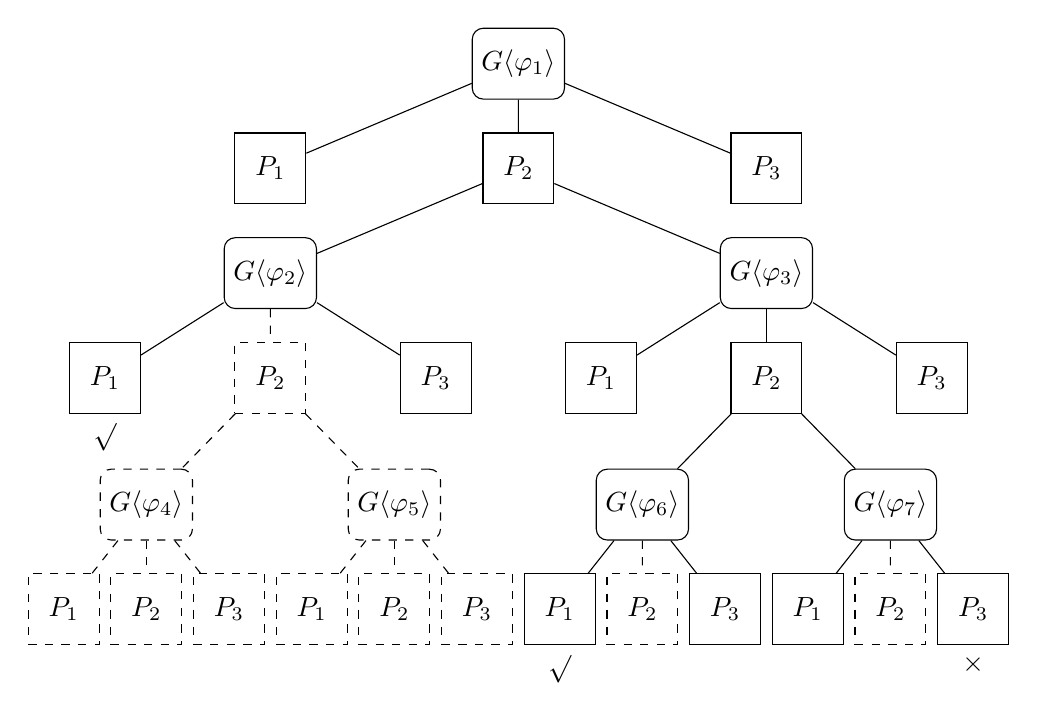
\begin{tikzpicture}[scale=0.7]
\tikzstyle{txt}=[scale=1.0]
\tikzstyle{succ}=[label=below:$\surd$]
\tikzstyle{fail}=[label=below:$\times$]
\tikzstyle{planbox}=[draw,minimum height=0.9cm,minimum width=0.9cm]
\tikzstyle{goalbox}=[draw,rounded corners,minimum height=0.9cm,minimum width=1.0cm]
\tikzstyle{level 1}=[sibling distance=4.5cm,level distance=1.9cm] 
\tikzstyle{level 2}=[sibling distance=9.0cm,level distance=1.9cm] 
\tikzstyle{level 3}=[sibling distance=3.0cm,level distance=1.9cm]
\tikzstyle{level 4}=[sibling distance=4.5cm,level distance=2.3cm]
\tikzstyle{level 5}=[sibling distance=1.5cm,level distance=1.9cm]
\tikzstyle{level 6}=[sibling distance=1.3cm,level distance=1.9cm]

\node[goalbox,yshift=1cm] {$G\langle\varphi_1\rangle$}
	child {node[planbox] {$P_1$}}
	child {node[planbox] {$P_2$}
		child {node[goalbox] {$G\langle\varphi_2\rangle$}
			child {node[planbox,succ] {$P_1$}}
			child[dashed] {node[planbox] {$P_2$}
				child {node[goalbox] {$G\langle\varphi_4\rangle$}
					child {node[planbox] {$P_1$}}
					child {node[planbox] {$P_2$}}
					child {node[planbox] {$P_3$}}
				}
				child {node[goalbox] {$G\langle\varphi_5\rangle$}
					child {node[planbox] {$P_1$}}
					child {node[planbox] {$P_2$}}
					child {node[planbox] {$P_3$}}
				}
			}
			child {node[planbox] {$P_3$}}
		}
		child {node[goalbox] {$G\langle\varphi_3\rangle$}
			child {node[planbox] {$P_1$}}
			child {node[planbox] {$P_2$}
				child {node[goalbox] {$G\langle\varphi_6\rangle$}
					child {node[planbox,succ] {$P_1$}}
					child[dashed] {node[planbox] {$P_2$}}
					child {node[planbox] {$P_3$}}
				}
				child {node[goalbox] {$G\langle\varphi_7\rangle$}
					child {node[planbox] {$P_1$}}
					child[dashed] {node[planbox] {$P_2$}}
					child {node[planbox,fail] {$P_3$}}
				}
			}
			child {node[planbox] {$P_3$}}
		}
	}
	child {node[planbox] {$P_3$}}
;

\end{tikzpicture}

}
\end{center}
\caption{Goal-plan hierarchy $\T_2$ containing a single goal type $G\langle\rangle$ handled by three plans $P_1$, $P_2$ and $P_3$. Here plan $P_2$ posts two instances of $G\langle\rangle$ resulting in recursion. Two levels of recursive unfolding are shown. Dashed $P_2$ nodes indicate roots of unexplored recursive sub-trees.}
\label{fig:unfolding}
\end{figure}

Consider the example BDI goal-plan hierarchy $\T_2$ of Figure \ref{fig:unfolding}. The structure has just a single event-goal type $G\langle\rangle$ and three options to handle it, one of which ($P_2$) in turn posts two instances of the same event-goal type $G\langle\rangle$. In this way, the only plans that take an action in the environment are $P_1$ and $P_3$. The figure highlights an execution trace as follows: \[
\lambda=G\langle\varphi_1\rangle[P_2:w_1] \cdot G\langle\varphi_2\rangle[P_1:w_1] \cdot G\langle\varphi_3\rangle[P_2:w_2] \cdot G\langle\varphi_6\rangle[P_1:w_2] \cdot G\langle\varphi_7\rangle[P_3:w_3].
\]

The first choice in the execution results in the selection of plan $P_2$ to handle event-goal instance $G\langle\varphi_1\rangle$ in a given world $w_1$. Plan $P_2$ in turn immediately posts the event-goal instance $G\langle\varphi_2\rangle$ that is successfully handled by the non-recursive node $P_1$. Plan $P_2$ then posts the second event-goal instance $G\langle\varphi_3\rangle$, which then is handled by itself in a recursive manner.  The outcome is that $\lambda$ traces a path that involves the successive execution of leaf plan $P_1$ for event-goal $G\langle\varphi_2\rangle$ followed by another execution of $P_1$ this time for event-goal $G\langle\varphi_6\rangle$, and finally terminates in the failure of leaf plan $P_3$ for event-goal $G\langle\varphi_7\rangle$. 

Note that if plan $P_2$ had instead been selected to handle $G\langle\varphi_7\rangle$ then a deeper recursive call would have ensued. Similarly if earlier in the execution trace plan $P_2$ was selected to handle event-goal $G\langle\varphi_2\rangle$ then a different recursive sub-tree (shown in Figure \ref{fig:unfolding} as dotted nodes under $G\langle\varphi_2\rangle$) would have unfolded.

The immediate implication of a recursive goal-plan structure is that the size of the hierarchy is no longer static but instead unfolds in a dynamic manner. The issue stems from the fact that the recursion is \textit{unbounded} because the context conditions that cause the recursion to terminate are initially unknown. So in order to know the context conditions we must recursively explore, but in doing so we risk an infinite recursive call because the context conditions that ought to guide the recursive exploration towards termination are unknown. This means that we may never find the ``bottom'' or leaf nodes. This has implications for any \textit{bottom-up} strategies. For instance, our conservative recording approach of \cite{Airiau:IJAT:09} and the coverage-based confidence measure of \cite{Singh:AAMAS10} both suffer from this problem. Interestingly, the simpler aggressive recording approach is not impacted by recursion as it does not consider the goal-plan structure . 

We will now focus on how the coverage-based confidence measure of \cite{Singh:AAMAS10} may be extended for use in recursive hierarchies.

\subsubsection{Calculating Coverage for Recursive Structures}

Since coverage is concerned with the number of paths {below} a plan in the goal-pplan hierarchy, then one way to interpret this for recursive structures is to treat all recursive goals simply as sub-trees in a static structure. Conceptually, this recursive unfolding of the structure is perfectly compatible with the coverage notion. 

Consider again the goal-plan structure $\T_2$ in Figure \ref{fig:unfolding} that shows the unfolding of the hierarchy for two levels of recursion. For the purpose of coverage calculations in this case, the three plans under each goal-event $G\langle\varphi_{4\ldots7}\rangle$ can be seen as having $[1,1,1]$ paths, plans under event-goals $G\langle\varphi_{2\ldots3}\rangle$ as having $[1,9,1]$ paths, and finally plans under $G\langle\varphi_1\rangle$ as having $[1,121,1]$ paths below.

The first difficulty with this reasoning, however, is that in fact the actual number of recursive unfoldings possible starting at $G\langle\varphi_1\rangle$ (or any other $G\langle\rangle$ for that matter) are \textit{infinite}. The only reason we are able to compute paths for structure $\T_2$ is because we have $bounded$ the recursion to a maximum of two levels.

It follows then that wherever a recursive structure applies and the coverage-based confidence measure is to be used, then a maximum recursion value must always be supplied. This may not be an unrealistic given that the domain expert will usually have some idea of how much recursion is sufficient, and as long as they provide a value that is sufficiently large for the domain then we have a valid case for computing coverage.

A second difficulty in this treatment of coverage is that the number of paths is exponential in the recursion number. For instance, in structure $\T_2$ in Figure \ref{fig:unfolding} the number of paths below $P_2$ for a progressively increasing recursion number is the series $[1, 9, 121, 15129, 228947161, \ldots]$. So within four levels of recursion, the number of paths below $P_2$ exceeds $228$ million.

Dhirendra says: Hmm.. one way to handle recursion would be to treat all recursive plans as \textit{leaf} nodes. This will enable coverage and stability to function in recursive domains ``as is''. Also all previous claims about coverage/stability will be preserved. Maybe this treatment of recursion makes more sense than bounded unfolding?!?

%Simplifications: Only single level goal recursion allowed ie G1->P1->G1 and not  G1->P1->G2->P2->G. Also no information of Gs in the system so only the parent goal recursion is tracked.

%\subsubsection{Discussion}
%Can we calculate $c_P(w,r)$ for any r if we have witnessed one r? 

%!TEX root = ../aamas11storage.tex
% %%%%%%%%%%%%%%%%%%%%%%%%%%%%%%%%%%%%%%%%%%%%%%%%%%%
\section{A Dynamic Confidence Measure}\label{sec:confidence}
% %%%%%%%%%%%%%%%%%%%%%%%%%%%%%%%%%%%%%%%%%%%%%%%%%%%

\Shout{Reword:Previous work has highlighted the importance of defining the exploration strategy for a general BDI learner in terms of it's goal-plan structure. The idea is that the extent of exploration of the structure in some way relates to our {\em confidence} in the resulting learning and may be used to construct the exploration heuristic. The notions of coverage \cite{singh10:learning} and structural complexity \cite{singh10:extending} both fall in this category. The benefit of these approaches is that they provide a monotonic confidence measure for guiding exploration (i.e. plan selection) in any general hierarchy. However, they use an estimate of the \textit{potential choices} below each node in the hierarchy, that may be difficult to calculate. Comparatively, the \textit{stability} \cite{airiau09:enhancing,singh10:learning} measure relies purely on {\em actual} plan execution and being independent of the hierarchy also scales well. However, stability does not have the same granularity as the former, so is not very useful for guiding exploration\footnote{In \cite{singh10:learning}, stability was used not as an exploration heuristic but as a filter to decide which experiences should be recorded for learning purposes.}. In this section, we describe a new confidence measure that combines the merits of the above approaches and overcomes their shortcomings. 

The stability-based confidence measure of Equation \ref{eqn:confidence} performs comparably to the proposed measures in \cite{singh10:learning,singh10:extending} in the respective domains used in those studies. So it serves as a direct replacement to the previous approaches. Moreover, the new measure improves upon the previous approaches in two key ways. Firstly, since the new stability-based measure is independent of the goal-plan structure in which it is used, then it is also truly scalable to practical applications. This factor was a key motivator for the work presented here.

Secondly, and importantly it addresses the case where the solution set being learnt is not fixed. For several online learning applications the solution space changes over time and the learner must re-learn as necessary. Here it is important for the agent to reliably recognise such changes, and respond by adjusting it's exploration policy, switching policies, choosing to start afresh, and so on. One way of identifying changes to the learnt solution space is by monitoring the ongoing performance of the agent, and reacting when a significant change is identified. Since the stability-based confidence measure relies on observed data (actual plan selection and outcome), it consequently reflects agent performance: our confidence is maximum when the observed performance is stable, and minimum when it is not. As such, the confidence measure may be directly used to build heuristics that dynamically adjust exploration against a variable solution set.}

To recap the definition of stability from \cite{singh10:learning}, ``A failed plan $P$ is considered to be stable for a particular world state $w$ if the rate of success of $P$ in $w$ is changing below a certain threshold $\epsilon$.'' Consider the example goal-plan structure of Figure \ref{fig:confidence} that shows the possible outcomes when plan $P$ is invoked in world state $w$. The $\surd$ and $\times$ symbols below the leaf plans indicate success and failure respectively. There is only one solution in world $w$ given by the sequential execution of the leaf plans $P_i$, $P_k$, and $P_m$. This is highlighted in Figure \ref{fig:confidence} as the shaded nodes. Line shading indicates initial execution traces while the solid shading highlights the final (active) execution trace. All other selection sequences lead to failures. Now let us consider the case where plan selection results in the failed active execution trace $\lambda_1=G[P:w] \cdot G1[P_a:w] \cdot G3[P_h:w]$. What should we make of this failure from a learning perspective? Should we record the negative sample for training our learners at non-leaf nodes $P_a$ and $P$? The concern stems from the fact that these non-leaf plans failed not because they were a bad choice for world $w$ but because a bad choice ($P_h$) was made further down in the hierarchy. The stability filter is used to resolve this issue in \cite{singh10:learning} by recording failures only for those plans that are considered to be stable, or ``well-informed''. 

Given the definition of stability, we now define the {\em degree of stability of failed node $N$ in world $w$ as the ratio of stable plans to total applicable plans in the active execution trace below $N$ and starting in $w$.} Here a node may be a plan or goal node. To see what this means, let us take the same failed trace $\lambda_1$ from before and say that $P_h$ is the only plan that is now stable. The degree of stability $s^o$ of each node in the trace $\lambda_1$ then is given by:

\begin{eqnarray*}
s^o(P_h,w) = & \frac{stable~in~[P_h]}{total~in~[P_h]} & = \frac{1}{1}  \\
s^o(G_3,w) = & \frac{stable~in~[P_g,P_h,P_i]}{total~in~[P_g,P_h,P_i]} & = \frac{1}{3}  \\
s^o(P_a,w) = & \frac{stable~in~[P_a,P_g,P_h,P_i]}{total~in~[P_a,P_g,P_h,P_i]} & = \frac{1}{4} \\
s^o(G_1,w) = & \frac{stable~in~[P_a,P_g,P_h,P_i,P_b,P_c]}{total~in~[P_a,P_g,P_h,P_i,P_b,P_c]} & = \frac{1}{6}  \\
s^o(P,w) = & \frac{stable~in~[P,P_a,P_g,P_h,P_i,P_b,P_c]}{total~in~[P,P_a,P_g,P_h,P_i,P_b,P_c]} & = \frac{1}{7} 
\end{eqnarray*}

Algorithm \ref{alg:degree} describes this calculation for any given active execution trace $\lambda$. Here $G_n[P_n:w_n,T_n]$ indicates that plan $P_n$ was executed in world $w_n$ to resolve goal $G_n$ where $T_n$ is the set of all applicable plans for the situation. The variables $s$ and $t$ store the number of stable and total plans respectively below $P_n$. $StablePlan$ is a function to check if the given plan $P_n$ is stable or not. Function $SetDegreeStability$ is used to save the degree of stability, given by the pair $s'/t'$, for each plan $P_n$.

\begin{algorithm}[ht]
\KwData{$\lambda=G_0[P_0:w_0,T_0] \cdot \ldots \cdot G_n[P_n:w_n,T_n]$; $s\geq0$; $t\geq0$; $k\geq0$; $\epsilon\geq0$}
\KwResult{Calculates the degree of stability for plans in $\lambda$}
\If{$|\lambda| > 1$}{
	$\lambda'=G_0[P_0:w_0] \cdot \ldots \cdot G_{n-1}[P_{n-1}:w_{n-1}]$\;
	$s' = s + StablePlan(P_n,w_n,k,\epsilon)$\;
	$t' = t + 1$\;
	$SetDegreeStability(P_n, w_n, s', t')$\;
	\ForEach{$P_i$ in $T_n$; $P_i \neq P_n$}{
		$s' = s' + StablePlan(P_i, w_n, k,\epsilon)$\;
		$t' = t + 1$\;
	}
	$UpdateDegreeStability(\lambda', s', t', k, \epsilon)$\;
}
\caption{$UpdateDegreeStability(\lambda, s, t, k, \epsilon)$}
\label{alg:degree}
\end{algorithm}

For our sample trace $\lambda_1$ for instance, the calculated $s^o(P,w)$ is $1/7$. The same measure for a different failed trace $\lambda_2=G[P:w] \cdot G1[P_b:w]$ where plan $P_b$ is the only stable plan would be $1/4$. Assuming all plans eventually become stable, $s^o(P,w)$ is guaranteed to converge to $1.0$. We use the {\em average degree of stability}, given by the average $s^o(P,w)$ over the last $n$ executions of plan $P$ in $w$, as a measure of our confidence in the decision tree for $P$ given $w$. Equation \ref{eqn:confidence-stability} defines this stability-based confidence measure $\C_s$ for plan $P$ over the last $n$ executions in world $w$ . This measure monotonically increases from $0.0$ as plans below $P$ start to become stable, and is $1.0$ when all tried plans below $P$ in the last $n$ executions are considered stable. 

\begin{equation}
\C_s(P,w,n) = \frac{s^o_0(P,w) + s^o_1(P,w) + \cdots + s^o_{n-1}(P,w)}{n}
\label{eqn:confidence-stability}
\end{equation}


The confidence measure $\C_s$ would make a useful heuristic for exploration (i.e. plan selection) in it's own right: such that when the confidence is at it's lowest we do maximum exploration and when it is at it's highest we fully utilise the decision tree. The problem with this approach, however, is that $\C_s$ only covers the space of known worlds. This means that whenever a new world is witnessed, $\C_s=0.0$, meaning that we will choose randomly. This is hardly beneficial since what we would really like is to use the learnt generalisations to classify this new world rather than be agnostic about it. What is missing is a metric that contributes to our net confidence but that is independent of $w$.

One way to achieve this is by monitoring the rate at which new worlds are being witnessed by the plan $P$. During early exploration it is expected that the majority of worlds that a plan is selected for will be unique, therefore this rate is high and our confidence is low. Over time as exploration continues, the plan would get selected in all possible worlds and the rate of new worlds would approach zero while our confidence over this period would increase to it's maximum.  Equation \ref{eqn:confidence-domain} defines this confidence metric $\C_d$ for plan $P$ over the last $n$ executions. Here, $W(P,*)$ is the set of all worlds witnessed by $P$ since the beginning and $\triangle W(P,n)$ is the set of worlds witnessed in the last $n$ executions. $\C_d$ is guaranteed to converge to $1.0$ as long as all worlds where the plan might apply are eventually witnessed.

\begin{equation}
\C_d(P,n) = \frac{|W(P,*)\cap \triangle W(P,n) |}{n}.
\label{eqn:confidence-domain}
\end{equation}

We are now ready to define our final confidence measure $\C$ based on the two component confidence metrics $\C_s$ and $\C_d$. Equation \ref{eqn:confidence} describes this calculation. Here $\alpha$ is the weighting factor used to set a preference bias between the two components.

\begin{equation}
\C(P,w,n) = (\C_s(P,w,n)*\alpha) + [\C_d(P,n)*(1.0-\alpha)].
\label{eqn:confidence}
\end{equation}

Finally, Equation \ref{eqn:omega} shows how the confidence measure $\C$ is used as a exploration heuristic during plan selection. Here $\P$ is the probability of success of plan $P$ in world $w$ as given by it's decision tree and $\Omega$ is the plan selection weight. This formulation of the plan selection weight is similar to those presented in \cite{singh10:extending, singh10:learning} bar the replacement of earlier measures with the new confidence term $\C$.

\begin{equation}
\Omega(P,w,n) = 0.5 + \left[  \C(P,w,n) *  \left( \P(P,w) - 0.5 \right)  \right]
\label{eqn:omega}   
\end{equation}


\Shout{Reword:Our example storage domain highlights the usefulness of this feature. Here, it is easy to think of situations where the solution space changes over time. For instance, our motivation for learning is that battery chemistry (and therefore performance) deteriorates over time, and the system should learn to avoid ideal solutions that no longer work in the future. However, old battery modules get replaced as and when required. So some ``solutions'' that the learner had eliminated previously now become applicable once again. Similar examples may be conjured for cases around module malfunctions. The point is that each such change in the environment impacts the solution space in some way. However, it is not assumed that an external signal is always available to notify us of these changes (some changes are continuous, for instance). Morevoer, several such factors may play on the solution space at one time, and it is up to the learner to respond in this environment appropriately.}

%!TEX root = ../ijcai11storage.tex
%%%%%%%%%%%%%%%%%%%%%%%%%%%%%%%%%%%%%%%%%%%%%%%%%%%%
\section{An Embedded Battery System Controller}\label{sec:application}
%%%%%%%%%%%%%%%%%%%%%%%%%%%%%%%%%%%%%%%%%%%%%%%%%%%%

\newcommand{\mmax}{\mathname{max}}

%Energy storage enables increasing levels of renewable energy in our electricity system, and the rapidly maturing supply chains for several battery technologies encourages electricity utilities, generators, and customers to consider using large battery systems. 
Large battery systems enable increasing levels of renewable energy in our electricity system. 
%
Such installations usually consist of multiple modules that can be controlled independently~\cite{norris02:grid}. 
%Often it is necessary to operate the modules in different states, such as if it is undesirable to change the direction of power flow too frequently, or due to battery technology requirements such as zinc-bromine flow batteries needing complete discharges at regular intervals. 
%Often it is necessary to operate the modules in different states, for instance due to battery technology requirements such as zinc-bromine flow batteries needing complete discharges at regular intervals. 
Since battery performance is susceptible to changes over time (e.g., modules may lose actual capacity) an \emph{adaptable} control mechanism is desirable that accounts for such changes.
%
Here, we describe an {\em embedded BDI controller for a modular battery system}, that regulates overall energy consumption of a smart office building comprise of loads (e.g., appliances) and generators (e.g., solar panels), by suitably ordering the battery to charge (i.e., act as a load) or discharge (i.e., act as a generator) at determined rates (the overall rate being the sum over the modules' rates).

Figure~\ref{fig:gptree} shows our implemented controller for an overall system capacity of $c$ (module capacity) $\times$ $k_{\mmax}$ (number of modules). Goal-event $G(r,k,s)$ requests a battery state (normalized) rate of $r \in [-1,1]$ (where $-1$ ($1$) indicates maximum discharge (charge) rate) by adjusting modules $[1,k]$ under current battery state $s$---initially, $k$ is set to $k_{\mmax}$. 
%%
The controller works by recursively configuring each module using plans $\pSetCharge$ (charge at rate $+c$), $\pSetDischarge$ (discharge at rate $-c$), and $\pSetNotUsed$ (disconnect, i.e., rate $0$), and after all modules have been configured, physically operating the battery for one period using the $\pExecute$ plan. 
%%

Observe that the first three plans contain known domain constraints for applicability using condition $\cSatisfies_X$. For instance, plan $\pSetCharge$ may not apply if the module is already charged; $\pSetDischarge$ may be ruled out if discharging the module means that no matter how the remaining modules are configured, the response will fall short of the request. When none of the plans apply, then BDI failure recovery is employed to backtrack and select a different configuration path until all constraints are satisfied or all options exhausted. 

Plan $\pExecute$ is therefore run only with functionally correct configurations. It first operates the whole battery for the period ($\aOperate$) and then evaluates the result via a sensor ($\aEvaluate$). If the evaluation \emph{succeeds}, then the desired rate $r$ has been met and the whole execution is deemed successful. Otherwise, the evaluation step \emph{fails} and so does the whole execution of the program, since no BDI failure recovery can be used after the battery system has been physically operated. 
%
Over time, the system learns the real applicability conditions of plans by training over their observed outcomes in different situations. In this way, programmed conditions act as an initial filter followed by learning
to decide final applicability.

%%%%%%%%%%%%%%%%%%%%%%%%%%%%%%%%%%%%%%%%%%%%%%%%%%%%
\subsection{Experimental Results}\label{sec:results}

All experiments used a battery system with five modules (i.e., $k_{\mmax}=5$). 
%
Each module had a charge state in the range $0$ (fully discharged) to $3$ (fully charged), as well as an assigned configuration for the period from $\{+c, 0, -c\}$, where $c=1/k_{\mmax}$.
%
%For each module, the current charge state is described by a discrete value in the range $[0:3]$, where zero indicates a fully discharged state and three indicates a fully charged state. In addition, each module has an assigned configuration for the current period from the set $\{+c, 0, -c\}$, where $c=1/k$. 
%
Charging adds $+c$ while discharging adds $-c$ to a module's charge state, otherwise the state is unchanged for the period (i.e., there is no charge loss). Thus, the net battery response is in the (normalized) range $[-1,1]$ in discrete intervals of $\pm c$. The state space for the problem is given by the modules ($5$), the requests ($11$), the charge states ($4^5$), and the assigned configurations ($3^5$), that is, $5 \times 11 \times 4^5 \times 3^5 \approx 13.7$ million. The agent does not learn over the full space, however, since the filtering of nonsensical configurations by the plans' context conditions $\cSatisfies_X(\cdot,\cdot,\cdot)$ reduces it substantially (to $\approx1.5$ million).
%
Each episode corresponds to one $G(r,5,s)$ goal-event request: achieve overall battery response of $r$ given current module charge states $s$.  For simplicity of analysis, we generate only satisfiable requests.
% i.e. a solution always exists. The outcome of each episode is either no response (no configuration was executed), or execution of the $\pExecute$ plan for operating (and evaluating) the battery. 
The threshold for stability calculation is set to $0.5$. We use an averaging window of $n=5$ for both the stability-based metric $\C_s$ and domain metric $\C_d$, and a (balanced) weighting of $\alpha=0.5$ for the final confidence measure $\C$.\footnote{Lower stability threshold gives greater accuracy (more samples) and vice versa. 
%$\alpha$ is generally not critical to performance.
$\alpha$ can be tuned towards $\C_d$ when the world is relatively complex compared to the structure of choices, or $\C_s$ otherwise.
} Each experiment is run five times and the reported results are averages from these runs. 
%
%Finally, in normal BDI operation, only plans that are deemed applicable as per their context condition are considered for execution. For our learning framework, where applicability is additionally defined by a plan's decision tree, this means that only plans with a reasonable likelihood of success should be allowed. To represent this, we used an \emph{applicability threshold} for plan selection of $40\%$, meaning that plans with a likelihood of success below this value are removed from consideration.\footnote{While this feature {\em does not alter the overall learning performance} of the battery controller, it does preclude the battery from being operated (i.e., plan $\pExecute$ being called) under module configurations that are likely to be unsuccessful. In fact, we found that the threshold used reduces the number of battery operations by $12\%$, which is substantial when considering battery life.}
Finally, since in normal BDI operation only plans deemed applicable as per their context condition are considered for execution, then for our learning framework we used an \emph{applicability threshold} of $40\%$, meaning that plans with a selection weight below this value are not considered.\footnote{The threshold does not alter overall performance, but does prevent battery use when it is unlikely to succeed. We found that it reduces operations by $12\%$, which is significant for battery life.}

The first experiment (Figure~\ref{fig:experiment1}) represents the traditional (one-off) learning setting. A deterioration in module capacities (at $\approx 5\kilo$ episodes) causes a rapid drop in performance (to $\approx 76\%$) corresponding to the set of programmed/learnt solutions that no longer work. Performance is subsequently rectified by learning to avoid configurations that no longer work. 
%The first experiment (Figure~\ref{fig:experiment1}) represents the traditional (one-off) learning setting where the agent recovers functionality against deterioration in module capacities (at around $5\kilo$ episodes). 
%
%%Typically this would occur over years of use, however to show the response to substantial change, we force this deterioration to occur instantaneously (at around $5\kilo$ episodes). 
%
%The resulting rapid drop in performance (to $\approx 76\%$ success) corresponding to the set of programmed/learnt solutions that no longer work, is subsequently rectified by the controller by learning to avoid configurations that no longer work. 
%
The next two experiments demonstrate adaptive behaviour when the environment dynamics is continually changing.
%
In Figure~\ref{fig:experiment2}, the agent is exposed to partial failures from modules malfunctioning (the first module fails during $[0,20\kilo]$ and is then restored, the second during $[20\kilo,40\kilo]$, and so on), but the battery remains capable of responding to requests using alternative configurations. The agent successfully learns to operate the battery without the failing module  each time.
%~\footnote{The apparent difference between performance drops at $0\kilo$ and $20\kilo$ is not meaningful in any way; it just happens that more ``bad'' cases occurred in the first failure.} 
%
Finally, in Figure~\ref{fig:experiment3}) the controller adapts in the extreme case of complete failure (during $[0,5\kilo]$).\footnote{Around $2\kilo$ episodes, the selection weight of {\em all} plans drops below the applicability threshold. To ensure that learning can still progress, we use as a ``soft'' applicability threshold mechanism: the $40\%$ threshold applies $90\%$ of the time.}
%
The key point in all experiments is that the learner does not require explicit notification of changes: it re-learns by adjusting exploration based on its performance (that reflects the impact of such changes).

%%%%%%%%%%%%%%%%%%%%%%%%%%%%%%%%%%%%%%%%%%%%%%%%%%%%
\section{Discussion and Conclusion}\label{sec:discussion}
%%%%%%%%%%%%%%%%%%%%%%%%%%%%%%%%%%%%%%%%%%%%%%%%%%%%

In this paper we propose a technique to enhance the typical plan selection
mechanism in BDI systems by allowing agents to learn and adapt the context
conditions of existing plans in the agent's plan library.
%%
As designing adequate context conditions that take full account of the agent's
environment for its complete life-cycle is often non-trivial, a framework that
allows for the \emph{refinement} of (initial) context conditions of plans
\textit{based on experience} is desirable. To this end we extend the BDI
framework to use \dt{}s as (part of) context conditions and provide a
probabilistic plan selection mechanism that caters for both exploration and
exploitation of plans.


We empirically evaluate two approaches to learning context conditions from experience, an aggressive approach that records and uses every outcome for learning, and a more conservative approach that records failure outcomes only when it considers the preceding choices that led to failure to be well-informed.
We confirm results from \cite{APSS08} that each approach has advantages in certain situations, but highlight an important shortcoming of the aggressive approach --- its complete inability to learn when applicability thresholds are used i.e. when the agent abandons plans with low chances of success. We then show that a new plan selection mechanism that also accounts for our confidence in the \dt\ classification can overcome the earlier issues with the aggressive approach. We conclude that the aggressive approach (that is also simpler), combined with the confidence measure (that also provides flexibility for tuning to different situations) is a better candidate for the general setting.

Our experiments do not consider the effects of conflicting interactions between sub-goals of a plan. For instance, if a sub-goal could succeed in more than one way causing different changes in the environment, one of which may in fact cause a subsequent sub-goal to fail, then in our current implementation it is not possible to detect and learn such interactions. Similarly we do not currently consider the effects of using failure recovery, under which alternative plans are tried upon the failure of a plan for achieving a goal. We note that both these features should be resolved for the real system. Moreover, we plan to do further experimentation with more realistic programs from existing applications. For continuous attributes, our approach requires that either the attributes be discretized or additional discrete attributes be used to test the continuous ones (for instance, check if temperature is $<20.5\textcelsius$).

One critique of the coverage-based confidence measure used is that it has a defined end state ($c_T(S)=1$) whereas for a real system, learning and re-learning will occur indefinitely as the agent continually tries to adapt to a changing environment. This implies that our confidence in a \dt's classification would also require calibration based on a changing environment. If the change in the environment was deliberate, then our confidence could be reset and subsequently \textit{re-built}. Without such an explicit signal the agent must rely on other methods for determining when the environment has changed significantly.

An appealing measure for recognising environmental changes is through the relatedness of its features. For instance, an observation that the grass is \textit{wet} presumably has a high correlation to the fact that it is \textit{raining}, and a \dt\ may (based on prior observations) very well use these factors in determining the likelihood of success of a plan to navigate the field. If then, we were to witness a world where it is not raining but the grass is wet (could be morning dew), then this world would be very different from the typical worlds we have seen so far and so we may have strong reason to reduce our confidence in the \dt\ classification of this new world.

The issue of combining learning and deliberative approaches for decision making in autonomous systems has not been widely addressed. In \cite{Riedmiller01} learning is used prior to deployment for acquiring low level robot soccer skills that are then treated as fixed methods in the deliberative decision making process once deployed. Hern\'andez et al. \cite{Hernandez04:Learning} give a preliminary account of how decision trees may be induced on plan failures in order to find an alternative logical context conditions in a deterministic paint-world example. More recently, in work related to BDI systems, \cite{Zhuo09:Learning} propose a method for learning hierarchical task network (HTN) method preconditions with partial observations in more complex domains. For this they first construct constraints from observed decomposition trees that are then solved offline using a constraint solver. In our work, learning and deliberation is integrated (as in \cite{APSS08}) such that one impacts the other and the classical exploration/exploitation dilemma applies. Initially, instead of following a random exploration policy (as is the case for agents with no initial knowledge), our agents are guided by the existing domain knowledge inherent in the BDI hierarchy.


%%%%%%%%%%%%%%%%%%%%%%%%%%%%%%%%%%%%%%%%%%%%%%%%%%%%


%ACKNOWLEDGMENTS are optional
\section{Acknowledgments}
We acknowledge the support of Agent Oriented Software and the Australian Research Council (under grant LP0882234).

%
% The following two commands are all you need in the
% initial runs of your .tex file to
% produce the bibliography for the citations in your paper.
\bibliographystyle{abbrv}
\bibliography{aamas11storage}

% You must have a proper ".bib" file
%  and remember to run:
% latex bibtex latex latex
% to resolve all references
%
% ACM needs 'a single self-contained file'!
%
%APPENDICES are optional
%\balancecolumns
%\appendix
%Appendix A
%\section{Headings in Appendices}

\end{document}
